\documentclass[a4paper]{article}

\usepackage[utf8]{inputenc}
\usepackage[T1]{fontenc}
\usepackage{textcomp}
\usepackage{listings}
\usepackage{lmodern}
\usepackage{amsfonts}
\usepackage{titling}
\usepackage{lipsum}
\usepackage[left=1in, right=1in, bottom=1in, top=1in]{geometry}
\usepackage{amsthm}
\usepackage{tcolorbox}
\usepackage{hyperref}
\usepackage{xcolor}
\usepackage{graphicx}
\usepackage{makeidx}
\usepackage{tikz}
\usepackage{cases}
\usepackage{apacite}
\usepackage{tkz-berge}
\usepackage{url}
\usepackage{tgtermes}
\usepackage{sectsty}
\usepackage{subcaption}
\usepackage{setspace}
\usepackage{float}
\usepackage{amsmath, amssymb}


% figure support
\usepackage{import}
\usepackage{xifthen}
\pdfminorversion=7
\usepackage{pdfpages}
\usepackage{transparent}
\usepackage{color}
\newcommand{\incfig}[2][1]{%
    \def\svgwidth{#1\columnwidth}
    \import{./figures/}{#2.pdf_tex}
}

%mathstyling
\theoremstyle{plain}
\newtheorem{thm}{Theorem}[section]
\newtheorem{lem}[thm]{Lemma}
\newtheorem{prop}[thm]{Proposition}
\newtheorem*{cor}{Corollary}

\theoremstyle{definition}
\newtheorem{defn}{Definition}[section]
\newtheorem{conj}{Conjecture}[section]
\newtheorem{exmp}{Example}[section]
\newtheorem{axiom}{Axiom}
\theoremstyle{remark}
\newtheorem*{rem}{Remark}
\newtheorem*{note}{Note}

\definecolor{darkgreen}{rgb}{0.0, 0.5, 0.0}

\pdfsuppresswarningpagegroup=1
\lstset{
tabsize = 4, %% set tab space width
showstringspaces = false, %% prevent space marking in strings, string is defined as the text that is generally printed directly to the console
numbers = left, %% display line numbers on the left
commentstyle = \color{darkgreen}, %% set comment color
keywordstyle = \color{blue}, %% set keyword color
stringstyle = \color{red}, %% set string color
rulecolor = \color{black}, %% set frame color to avoid being affected by text color
basicstyle = \small \ttfamily , %% set listing font and size
breaklines = true, %% enable line breaking
numberstyle = \tiny,
  frame=none,
  xleftmargin=2pt,
  stepnumber=1,
  belowcaptionskip=\bigskipamount,
  captionpos=b,
  escapeinside={*'}{'*},
  language=haskell,
  tabsize=2,
  emphstyle={\bf},
  showspaces=false,
  columns=flexible,
  showstringspaces=false,
  morecomment=[l]\%,
}
\begin{document}
	\begin{titlepage}
	\begin{center}
	\large
	University of Warwick \\
	Department of Computer Science \\
	\huge
	\vspace{50mm}
	\rule{\linewidth}{0.5pt} \\
	CS255 \\
	\vspace{5mm}
	\Large
	Artificial Intelligence
	\rule{\linewidth}{0.5pt}
	\vspace{5mm}
	\begin{figure}[H]
	\centering
	
\includegraphics[width=0.4\textwidth]{crest_black.eps}
	\end{figure}
	\vspace{37mm}
	Cem Yilmaz \\
	\today
	\end{center}
	\end{titlepage}
	\tableofcontents
	\newpage
	\section{Agents}
	\begin{tcolorbox}[colback=black!3!white,colframe=black!60!white,title=\begin{defn}Agent \label{Agent}\end{defn}]
	An agent is an entity that perceives and acts. An agent can be viewed as a function from percept histories to actions, where
	\begin{align*}
		f : P \to A
	\end{align*}
	\end{tcolorbox}
	Agents typically required at exhibit autonomy. For any given class of environments and tasks we seek the agent(s) with the best performance. Perfect rationality usually impractical given computational restraints, therefore, it is the best that we design the best agent for a given set of resources.
	\begin{tcolorbox}[colback=black!3!white,colframe=black!60!white,title=\begin{defn}Artifical Intelligence \label{Artificial Intelligence}\end{deft}]
	Artificial intelligence is the synthesis and analysis of computational agents that act intelligently. An agent acts "intelligently" if:
	\begin{itemize}
		\item its actions are appropriate for its goals and circumstances
		\item it is flexible to changing environments and goals
		\item it learns from experience
		\item it makes appropriate choices given its perceptual and computational limitations
	\end{itemize}
	\end{tcolorbox}
	However, note that artificial intelligence has different goals: \\
\textbf{Scientific Goal}: to understand the principles that make intelligence behaviour possible in natural or artificial systems. That is, analyse natural and artificial agents, formulate and test hypotheses about what it takes to construct intelligent agents and finally design, build and experiment with computational systems that perform tasks that require intelligence\\
\textbf{Engineering Goal:} design useful, intelligence artefacts \\
For this module, the main goal is engineering goal. \\
\subsection{Inputs to an agent}
There are several inputs to an agent, that list as following:
\begin{enumerate}
	\item Abilities - the set of possible actions it can perform
	\item Goals/Preferences - what it wants, its desires, its values ...
	\item Prior Knowledge - what it comes into being knowing, what it doesn't get from experience, ...
	\item History of stimuli - what it has received in the past. However, current stimuli is what it perceives from environment now.
\end{enumerate}
However, note that rational $\neq $ omniscient. An omniscient agent would know the actual outcome of its actions - agents are rarely omniscient since unexpected situations occur in dynamic environments. A rational agent needs only to do its best given the current percepts. Similarly, rational $\neq $ clairvoyant. An agent is not expected to foresee changes in its environment. Lastly, rational $\neq $ successful. Rational action is defined in terms of expected value, rather than actual value; a failed action can still be rational. \\
\subsection{Dimensions of Complexity}
	\subsubsection{Modularity}
	Agent structure has one level of abstraction: flat. Agent structure has interesting modules that can be understood separately: modular. Agent structures has modules that are decomposed into modules: hierarchical. \\
	\subsubsection{Planning Horizon}
	Planning horizon is how far the agents look into the future when deciding what to do. A static is a non-planning AI. Finite stage are agent reasons about a fixed number of time steps. Indefinite stage are agent reasons about a finite, but not predetermined, number of steps. Infinite stage is the case that agent plans for going on forever.\\
	\subsubsection{Representation}
	Much of modern AI is about finding compact representations and exploiting the compactness for computational gains. An agent can reason in terms of explicit states, where a state is one way the world could be, features and propositions where states can be described using features, and finally, individuals and relations where there is a feature for each relationship on each tuple and individual. 
\subsubsection{Learning from experience}
Whether the model is fully specified a priori: knowledge is given or knowledge is learned from data or past experience.
\subsubsection{Uncertainty}
There are two dimensions for uncertainty - sensing and effect. In each dimension an agent can have no uncertainty, disjunctive uncertainty or probabilistic uncertainty. Usually we would choose probability as agents can still act even if they are uncertain. Predictions are needed to decide what to do. Acting is gambling - agents who do not use probability will lose to those that do, and probabilities can be learned from data and prior knowledge.
\subsubsection{Sensing Uncertainty}
\subsubsection{Effect Uncertainty}
A deterministic environment is the resulting state is determined from the action and the state. Stochastic is there is uncertainty about the resulting state.
\subsubsection{Preferences}
An agent has achievement goal to achieve - this can a complex logical formula. Complex preferences may involve trade-offs between various desiderata, perhaps at different times from ordinal and cardinal. Ordinal is where only the order matters, and cardinal is where the values also matter.
\subsubsection{Number of Agents}
Are there multiple reasoning agents that need to be taken into account? Single agent reasoning - any other agents are part of the environment. Or multiple agents, an agent reasons strategically about the reasoning of other agents. Agents can have their own goals - cooperative, competitive, or goals can be independent of each other
\subsubsection{Interaction}
When does the agent reason to determine what it do? Reason offline - before acting or reason online - while interacting with the environment
\section{Representation}
We want a representation to be
\begin{itemize}
	\item rich enough to express the knowledge needed to solve the problem
	\item as close to the problem as possible - compact, natural and maintainable
	\item amenable to efficient computation i.e., able to express features of the problem that can be exploited for computational gain or able to trade off accuracy and computation time and/or space.
	\item Able to be acquired from people, data and past experiences.
\end{itemize}
\subsection{Defining a solution}
Given an informal description of a problem what is a solution? Typically much is left unspecified, but the unspecified parts cannot be filled arbitrarily. Much work in AI is motivated by common-sense reasoning - the computer needs to make common-sense conclusions about the unstated assumptions. What matters too, is the quality of solutions -
\begin{itemize}
	\item An optimal solution - is a best solution according some measure of quality
	\item Satisfying solution - is one that is enough, according to some description of which solutions are adequate
	\item Approximately optimal solution - is one whose measure of quality is closer to the best theoretically possible
	\item Probable solution - one that is likely to be a solution
\end{itemize}
\subsection{Decisions and outcome}
Good decisions can have bad outcomes and equally bad decisions can have good outcomes. Information can be valuable because it leads to better decisions: can sometimes quantify the value of information. We can often trade off computation time and solution quality. An anytime algorithm can provide a solution at any time; given more it can produce better solutions. An agent is not just concerned about finding he right answer, but about acquiring the appropriate information, and computing it in a timely manner.
\subsection{Physical Symbol System Hypothesis}
A symbol is a meaningful physical pattern that can be manipulated. A symbol system creates, copies, modifies and destroys symbols. A physical symbol system hypothesis has the necessary and sufficient means for general intelligent action.
\begin{itemize}
	\item The knowledge level is in terms of what an agent knows and what its goals are
	\item The symbol level is a level of description of an agent in terms of what reasoning it is doing
\end{itemize}
to map from problem to representation, we need to think about level of abstraction the problem represents, what individuals and relations in the world to present, how can an agent represent the knowledge to ensure that the representation is natural, modular and maintainable, how can an agent acquire the information from data, sensing experience or other agents
\subsection{Knowledge and Symbol Levels}
Two levels of abstraction seem to be common among biological and computational entities: the knowledge level is in terms of what an agent knows and what its goals are. The symbol level is a level of description of an agent in terms of what reasoning it is doing.
\subsection{Agent System Architecture}
\begin{figure}[H]
	\centering
	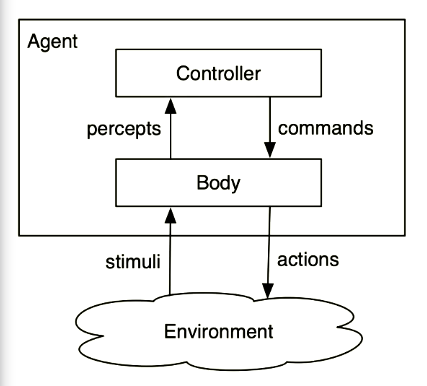
\includegraphics[width=0.5\textwidth]{1.png}
	\caption{Agent System Architecutre}
	\label{fig:1-png}
\end{figure}
An agent interacts with the environment through its body. The body is made up of sensors that interpret stimuli and actuators that carry out actions. The controller receives percepts from the body and the controller sends commands to the body. The body can also have reactions that are not controlled.
\subsection{Controller}
A controller is the brains of the agent. Agents are situated in time, they receive sensory data in time and do actions in time. Controllers have limited memory and limited computational capabilities. The controller specifies the command at every time. The command at any time can depend on the current and previous concepts. For agent of functions, let $T$ be the set of time points. A percept trace is a sequence of all past, present and future percepts received the controller. A command trace is similar but with commands except of percepts. A transduction is a function from perept traces into command traces. A transduction is causal if the command trace up up to time $t$ depends only on percepts up to $t$. A controller is an implementation of the causal transduction. An agent's history at time $t$ is a sequence of past and present percepts and past commands. A causal transduction specifies a function from an agent's history at time $t$ into its action at time $t$.
\subsection{Belief States}
An agent does not have access to its entire history, it only has access to what it has remembered. The memory or belief state of an agent at time $t$ encodes all of the agent's that it has access to. The belief state of an agent encapsulates the information about its past it can use for current and future actions. At every time a controller has to decide what it should do, what should it remember and how should it update its memory. This is a function of its percepts and its memory. For discrete time, a controller implements
\begin{itemize}
	\item belief state function - remember(belief state, percept). Returns the next belief state
	\item command function - do(memory, percept). Returns the command for an agent
\end{itemize}
\begin{figure}[H]
	\centering
	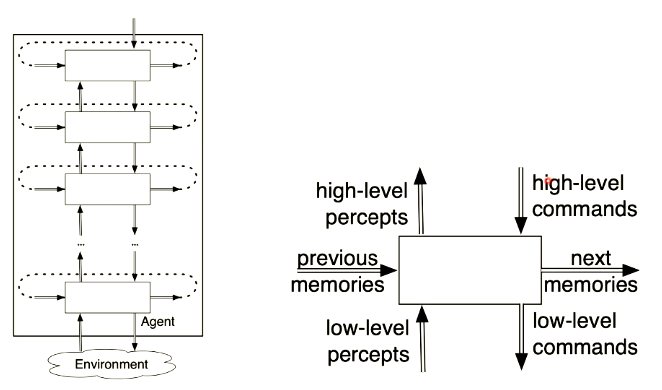
\includegraphics[width=0.6\textwidth]{2.png}
	\caption{Hierarchical Robotic System Architecture}
	\label{fig:2-png}
\end{figure}
The layer above generally begins abstract e.g., travelling to a destination using a car. However, by the time the architecture arrives to the bottom layer. For example, pedestrian avoidance, pedestrian detection, etc. The commands may also change depending on their level of abstraction. The functions implemented a layer are described as
\begin{itemize}
	\item remember(memory, percept, command) - we need to take command that comes down from higher level
	\item do(memory, percept, command) - we may need to modify the command depending on memory and perception that is received
	\item higher$\_$percept(memory, percept, command) - we need to decide which perceptions we need to pass back up depending on our memory and command (which may have changed from the bottom layer and now we are sending it back to the layer above)
\end{itemize}
\begin{tcolorbox}[colback=black!3!white,colframe=black!60!white,title=\begin{exmp}Delivery Robot \label{Delivery Robot}\end{exmp}]
        The robot has three actions: go forward, right or left.\\
	It can be given a plan consisting of a sequence of named locations for the robot to go to in turn. The robot must avoid obstacles. It has a single whisker snesor pointing forward and to the right. The robot can detect if the whisker hits an object and the robot knows its current location. The obstacles and locations can be moved dynamically; obstacles and new locations can also be created dynamically
	\begin{figure}[H]
		\centering
		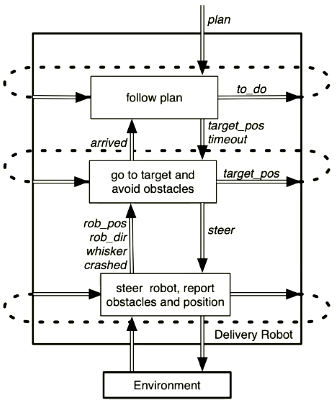
\includegraphics[width=0.4\textwidth]{3.png}
		\caption{Architecture of the example}
		\label{fig:3-png}
	\end{figure}
\end{tcolorbox}
To decide what should be in an agent's belief state, we need to first determine what kind of an agent it is. We know that a purely reactive agent does not have a belief state, and a dead reckoning agent does not perceive the state. Neither work well in complicated domains, but were proven to be useful in simple situations. It is often useful for the agent's belief state to be a model of the world. \\
\begin{tcolorbox}[colback=black!3!white,colframe=black!60!white,title=\begin{defn}Ideal Rational Agent \label{Ideal Rational Agent}\end{defn}]
Does whatever action is expected to maximise performance measure on basis of percept sequence and built-in knowledge
\end{tcolorbox}
Therefore, in theory ideal mapping of percept sequences to actions correspond to an ideal agent. The simplest approach is a lookup table. However, this fails because the size is too big, the time to build is too high, and has no autonomy. Nevertheless, the table suggests a notional ideal mapping. One agent function (or a small equivalence class) is rational. Our aim is to find a way to implement the rational agent function. We need to implement rational agent function concisely. The implementation must be relatively efficient, exhibit autonomy if required and get as close as possible to the ideal mapping. 
\subsection{Agent Types}
\begin{tcolorbox}[colback=black!3!white,colframe=black!60!white,title=\begin{defn}Simple Reflex Agents \label{Simple Reflex Agents}\end{defn}]
These are condition action rules. More precisely, this is the if then statement.
\end{tcolorbox}
\begin{tcolorbox}[colback=black!3!white,colframe=black!60!white,title=\begin{defn}Reflex agents with state \label{Reflex agents with state}\end{defn}]
This agent retains the knowledge about the world e.g., the output of the action. 
\begin{figure}[H]
	\centering
	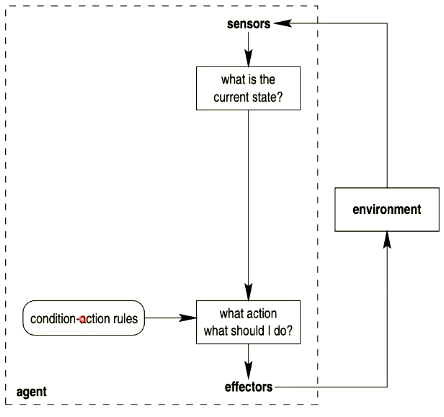
\includegraphics[width=0.5\textwidth]{4.png}
	\caption{Reflex Agent}
	\label{fig:4-png}
\end{figure}
Note that sensors are the only thing that show the agent's current state which are determined by the sensors. We can modify the diagram above to include a state that can help it enhance its decisions depending on its percept state.
\begin{figure}[H]
	\centering
	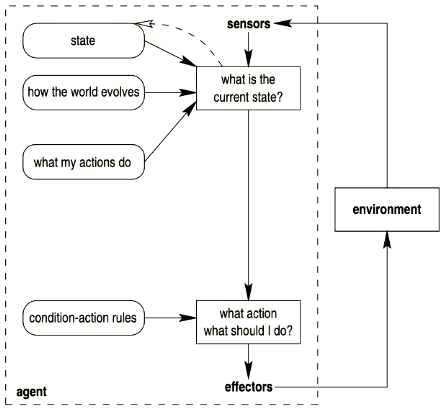
\includegraphics[width=0.5\textwidth]{5.png}
	\caption{State Reflex Agent}
	\label{fig:5-png}
\end{figure}
\end{tcolorbox}
\begin{tcolorbox}[colback=black!3!white,colframe=black!60!white,title=\begin{defn}Goal-based agents \label{Goal-based agents}\end{defn}]
This has representation of what states are desirable
\begin{figure}[H]
	\centering
	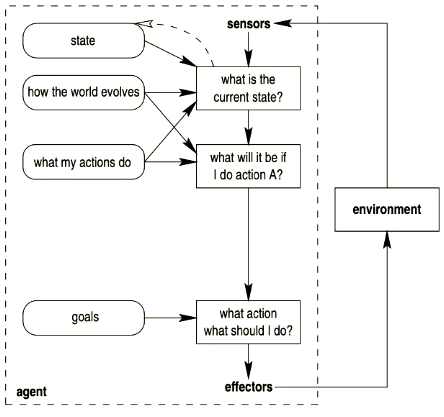
\includegraphics[width=0.5\textwidth]{6.png}
	\caption{Goal-based agent}
	\label{fig:6-png}
\end{figure}
The main change of this agent is the question "what will it be if I do action $A$"? The complexity of this agent increases substantially.
\end{tcolorbox}
\begin{tcolorbox}[colback=black!3!white,colframe=black!60!white,title=\begin{defn}Utility-based agents \label{Utility-based agents}\end{defn}]
Ability to discern some useful measure e.g., cost, quality between possible means of achieving some state. 
\begin{figure}[H]
	\centering
	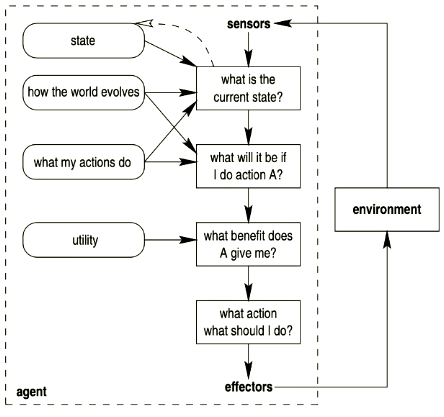
\includegraphics[width=0.5\textwidth]{7.png}
	\caption{Utility-based agent}
	\label{fig:7-png}
\end{figure}
We focus on utility and the benefits separately rather than searching for a win state when making our decision. The utility function also enables a choice about which goals to achieve - we select the one with the highest utility. If achievement is uncertain we can measure the importance of goal against likelihood achievement.
\end{tcolorbox}
\begin{tcolorbox}[colback=black!3!white,colframe=black!60!white,title=\begin{defn}Learning agents \label{Learning agents}\end{defn}]
Able to modify their behaviour based on their performance, or in the light of new information
\begin{figure}[H]
	\centering
	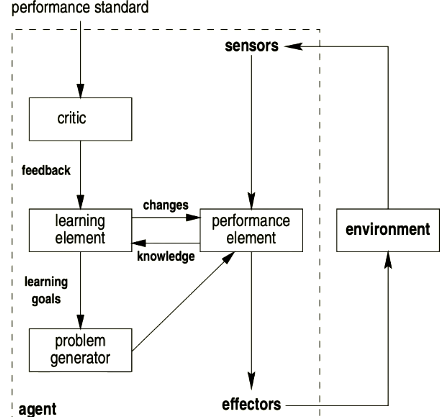
\includegraphics[width=0.5\textwidth]{8.png}
	\caption{Learning Agent}
	\label{fig:8-png}
\end{figure}
	Learning agent gradually modifies itself. Typically we have objectives that generates problems that feeds into the performance element. We then find out whether our problem solving went well or not. It is then fed back to learning element and looped. The critic and the performance standard tells how well the AI did after using the problem. 
\end{tcolorbox}

\end{document}
